%%% Preamble
\documentclass[paper=a4, fontsize=11pt]{scrartcl}
\usepackage[utf8]{inputenc}

\usepackage{fourier}

\usepackage[german]{babel}
\usepackage[protrusion=true,expansion=true]{microtype}	
\usepackage{amsmath,amsfonts,amsthm} % Math packages
\usepackage[pdftex]{graphicx}	
\usepackage{url}


%%% Custom sectioning
\usepackage{sectsty}
\allsectionsfont{\centering \normalfont\scshape}

%%% European newline
\setlength{\parindent}{0pt}
\setlength{\parskip}{4pt}

%%% Custom headers/footers (fancyhdr package)
\usepackage{fancyhdr}
\pagestyle{fancyplain}
\fancyhead{}											% No page header
\fancyfoot[L]{}											% Empty 
\fancyfoot[C]{}											% Empty
\fancyfoot[R]{\thepage}									% Pagenumbering
\renewcommand{\headrulewidth}{0pt}			% Remove header underlines
\renewcommand{\footrulewidth}{0pt}				% Remove footer underlines
\setlength{\headheight}{13.6pt}


%%% Equation and float numbering
\numberwithin{equation}{section}		% Equationnumbering: section.eq#
\numberwithin{figure}{section}			% Figurenumbering: section.fig#
\numberwithin{table}{section}				% Tablenumbering: section.tab#


%%% Maketitle metadata
\newcommand{\horrule}[1]{\rule{\linewidth}{#1}} 	% Horizontal rule

\title{
	%\vspace{-1in} 	
	\usefont{OT1}{bch}{b}{n}
	\normalfont \normalsize \textsc{MNG} \\ [25pt]
	\horrule{0.5pt} \\[0.4cm]
	\huge Programmieren eines Spiels in Java \\
	\horrule{2pt} \\[0.5cm]
}
\author{
	\normalfont 								\normalsize
	Max Mathys\\[-3pt]		\normalsize
	\today
}
\date{}


%%% Begin document
\begin{document}
	\maketitle
	\section{Einleitung}
	
	Für dieses Projekt wurde ein Spiel in Java programmiert, bei dem Aktien gehandelt werden können. Das Ziel des Spiels ist es, dass man möglichst viel Geld generiert.
	
	Die Steuerung des Spiels wird durch die Interaktion im Terminal ermöglicht.
	
	Das Ziel dieses Projektes ist die OOP-Kenntnisse in Java selbstständig anzuwenden und so eine praxisorientierte Kenntnis von OOP zu erlangen.
	
	\section{Struktur}
	
	Die Applikation wurde so programmiert, dass die Prinzipien der Objektorientierung angewendet werden.
	
	Die wichtigsten Klassen sind Abbildung \ref{fig:uml} dargestellt.
	
	\begin{itemize}
		\item Ein gestrichelte Linie bedeutet, dass die Klassen die entsprechende Klasse im Code verwenden.
		\item Es wurden nicht alle Referenzen (welche anderen Klassen eine Klasse verwendet)  eingezeichnet, sondern nur die wichtigsten.
		\item Eine durchgezogene Linie bedeutet, dass die Klasse von der anderen abstammt. Hierbei ist immer die untere Klasse das Kind.
		\item Statische Funktionen werden unterstrichen.
		\item Für eine verbesserte Übersicht werden private Funktionen und alle Attribute nicht dargestellt.
		
	\end{itemize}
	
	\begin{figure}[!htbp]
		\centering
		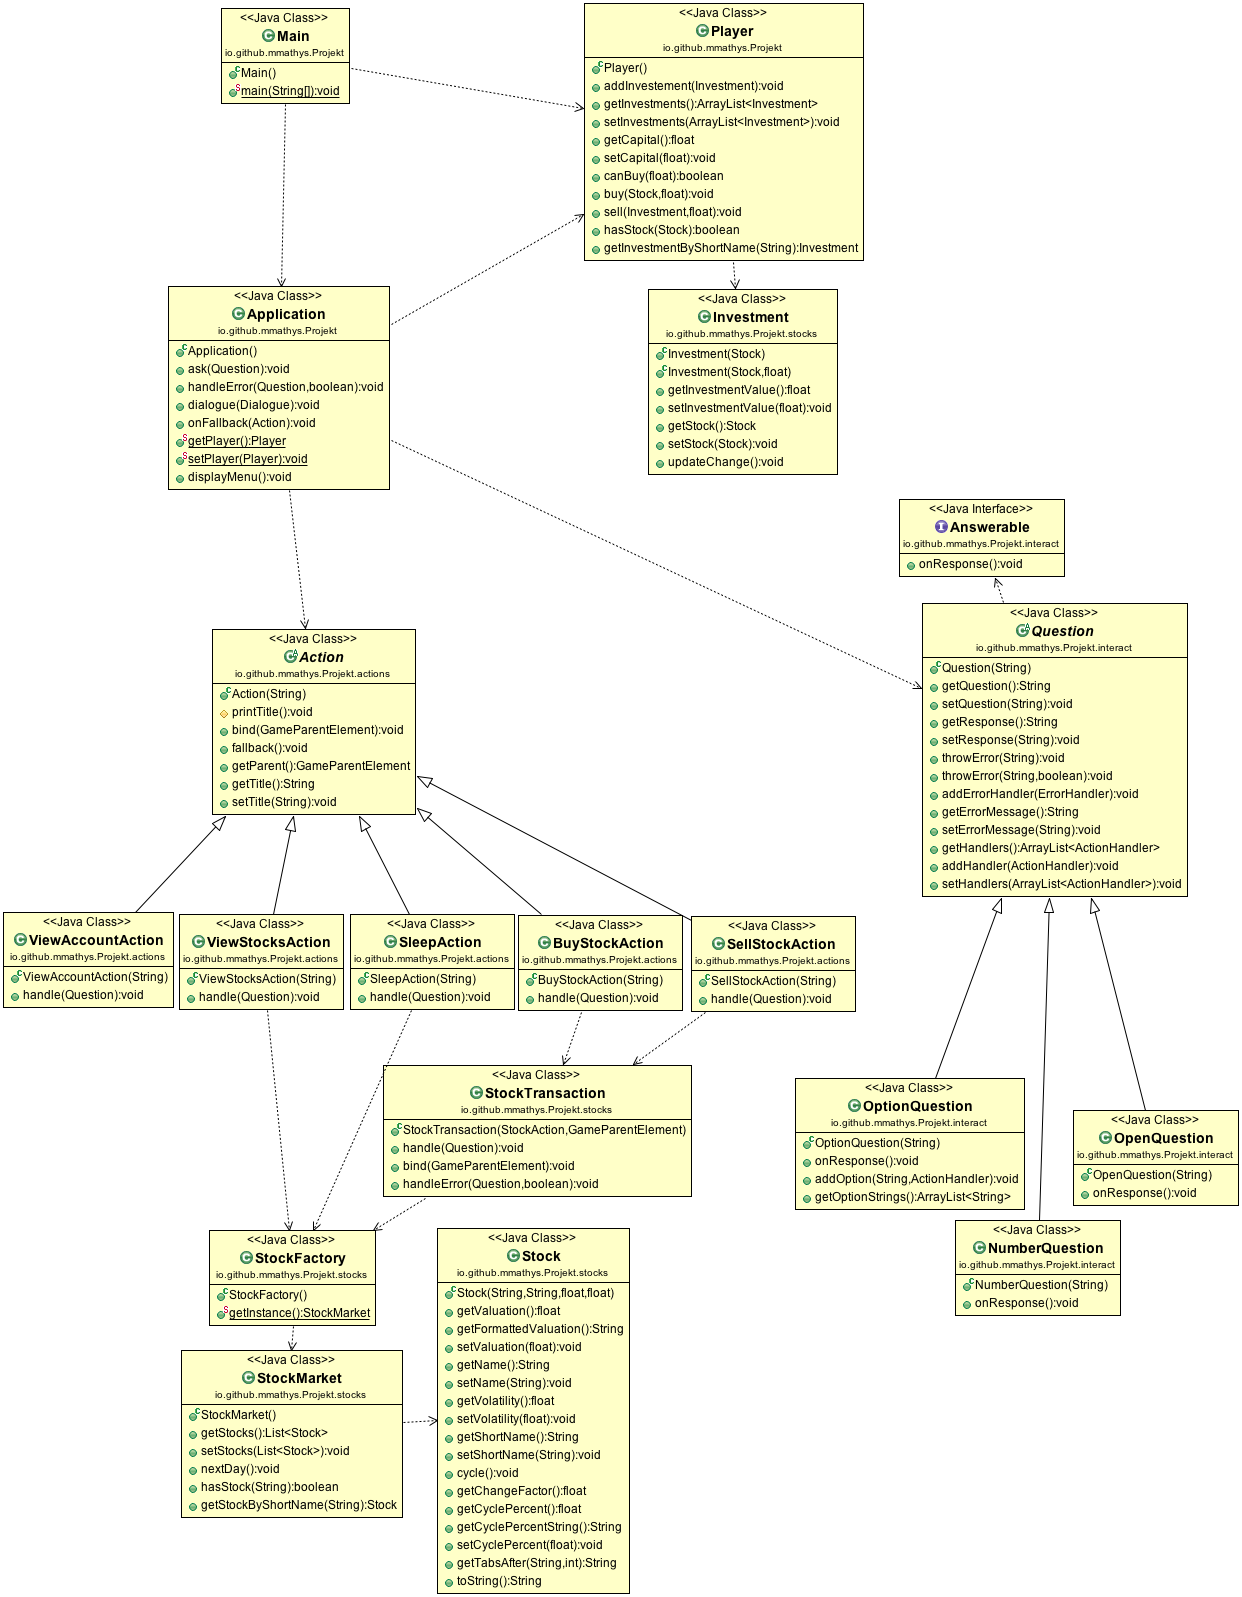
\includegraphics[width=\linewidth]{UML1}
		\caption{UML-Diagramm}
		\label{fig:uml}
	\end{figure}
	
	\paragraph{Main.} Hier wird die Applikation gestartet. Es werden Instanzen der Applikation und Spieler erstellt.
	
	\paragraph{Player.} Diese Klasse stellt den Spieler dar. Er besitzt Attribute wie das Kapital oder die gekauften Aktien. Zudem verfügt der Spieler über Kauf- und Verkaufsfunktionen für Aktien.
	
	Obwohl es nur eine Instanz des Spielers im Programm gibt, ist er nicht statisch: Es wurde entschieden, dass nur der Spieler-Accessor in \texttt{Application} statisch sein sollte.
	
	\paragraph{Application.} Diese Klasse ist das Kernstück des Programms: Von dieser Klasse gehen alle Aktionen im Spiel aus. Es kann das Menü anzeigen, Fragen stellen, Dialoge führen und Fehler anzeigen.
	
	\paragraph{Action und Kinder.} Wenn das Konto aufgerufen, Aktien betrachtet, gekauft oder verkauft oder geschlafen werden will, so wird über das Menü in \texttt{Application} eine bestimmte \texttt{Action} aufgerufen.
	
	Das \texttt{Action} eine abstrakte Klasse ist, kann sie nicht direkt aufgerufen werden, sondern nur ihre Kinder \texttt{ViewAccountAction}, \texttt{ViewStocksAction}, \texttt{BuyStocksAction}, \texttt{SellStocksAction} und \texttt{SleepAction}. 
	
	\texttt{ViewAccountAction}, \texttt{ViewStocksAction}, \texttt{BuyStocksAction} und \texttt{SellStocksAction} haben alle direkt oder indirekt mit Aktien zu tun: Sie benützen alle die Stock-Klassen (\texttt{StockFactory}, \texttt{StockTransaction}, \texttt{StockMarket} und \texttt{Stock}).
	
	\texttt{ViewAccountAction} zeigt Informationen zum Spieler an.
	
	\paragraph{Stock-Klassen}
	
	\texttt{StockFactory}, \texttt{StockTransaction}, \texttt{StockMarket} und \texttt{Stock} werden als \textit{Stock-Klassen} bezeichnet.
	
	Durch die \texttt{StockFactory} kann durch eine statische Funktion die Instanz des \texttt{StockMarkets} aus jeder anderen Klasse geholt werden. Die Klasse \texttt{StockMarket} beinhaltet die Aktien und aktualisiert deren Kurse.
	
	Die Klasse \texttt{Stock} stellt eine Aktie dar. Sie enthält Attribute wie der Gesamtwert der Firma, Name, Kürzel, Schwankungsfreudigkeit oder Änderung des Kurses.
	
	Wenn der Spieler eine Aktie kaufen oder verkaufen will, kommt die Klasse \texttt{StockTransaction} ins Spiel. Sie implementiert die Programmlogik für \texttt{BuyStockAction} und \texttt{SellStockAction}.
	
	\paragraph{Question}
	
	Die Kinder der \texttt{Question}-Klasse implementieren das Fragen im Programm. Es kann nach Zahlen oder nach Strings gefragt werden.
	
	\texttt{OptionQuestion} wird beim Menü verwendet. Der Nutzer kann aus Optionen auswählen.
	
	\texttt{NumberQuestion} fragt nach Float-Zahlen.
	
	\texttt{OpenQuestion} erlaubt eine Antwort beliebiger Zeichenstrings, wie zum Beispiel nach einem Aktienkürzel.
	
	\section{Implementierung}
	
	\paragraph{Schwankung von Aktien.} Der Wert, Name, Kürzel und Schwankung der Aktien wurden in einem Array in einer Java-Klasse als statische finale Variablen gespeichert. Nach jedem Tag im Spiel wird der Wert der Aktien neu berechnet. Dazu wurde zu jeder Aktie die Schwankungsfreudigkeit von 0 bis 1 definiert. Bei 1 ist die maximal mögliche Schwankung 100\%, bei 0 0\%.
	
	\paragraph{Zugriff von Aktionsklassen auf \texttt{Application}.} Damit Klassen wie \texttt{Question}, \texttt{Action} oder \texttt{StockTransaction} ebenfalls fragen stellen können, werden sie mit einer \texttt{bind()}-Funktion ausgestattet, damit eine Instanz von \texttt{Application} übergeben werden kann.
	
	So können diese Klassen so Fragen stellen, Fehler ausgeben und nach Abschliessung ihrer Funktion ein \textit{Callback} geben (damit die Applikation zu ihrem ursprünglichen Zustand, zum Menü, zurückkehrt).
	
	\paragraph{ASCII-Unterstützung.} ASCII nennt man die Technik, die in Terminals verwendet wird, falls Farben, Durchstreichungen, Unterstreichungen und ähnliches verwendet werden will.
	
	Falls kein ASCII im Terminal angezeigt werden kann, wird am Anfang des Spiels eine Fehlermeldung ausgegeben. Da man nicht programmatisch prüfen kann, ob der Terminal ASCII-fähig ist, wird folgende Strategie verwendet: Die Textfarbe der Fehlermeldung ist gleich wie sein Hintergrund und wird bei jedem Start der Applikation ausgegeben. Falls kein ASCII unterstützt wird, wird die Fehlermeldung sichtbar.
	
	\section{Funktionsweise des Spiels}
	
	Im Spiel wird man in die Rolle eines Brokers an der NYSE versetzt. Am Anfang spricht man mit seinem Manager, der einem das Geschäft erklärt.
	
	Anschliessend kann man zwischen folgenden Aktionen auswählen:
	
	\begin{itemize}
		\item{Konto ansehen}
		\item{Aktienmarkt betrachten}
		\item{Aktie kaufen}
		\item{Aktie verkaufen}
		\item{Schlafen gehen}
	\end{itemize}
	
	\paragraph{Konto ansehen}
	
	Das Konto zeigt das Kapital und die gekauften Aktien des Spielers an. Je nach Spielstand bekommt er ein Feedback seines Chefs.
	
	\paragraph{Aktienmarkt betrachten}
	
	Beim Aktienmarkt wird die Aktienmarkt-Tafel angezeigt, wo alle verfügbaren Aktien aufgelistet sind. Zum Namen wird der Kürzel angezeigt, auch die Änderung einer Aktie während einem Tag. Zum Schluss wird noch der Gesamtwert der Aktie aufgelistet.
	
	\paragraph{Aktie kaufen / Aktie verkaufen}	
	
	Wenn der Spieler eine Aktie kaufen oder verkaufen will, muss er zuerst den Aktienkürzel angeben und danach den Wert der Transaktion.
	
	\paragraph{Schlafen gehen}
	
	Wenn der Spieler schlafen geht, beginnt ein neuer Tag an der Aktienbörse: Die Aktienkurse verändern sich. 
	
	\section{Schlussfolgerung}
	
	
	
\end{document}